\documentclass[a4paper,12pt]{article}

\usepackage[14pt]{extsizes}
\usepackage{cmap}					% поиск в PDF
\usepackage{mathtext} 				% русские буквы в формулах
\usepackage[T2A]{fontenc}			% кодировка
\usepackage[utf8]{inputenc}			% кодировка исходного текста
\usepackage[english,russian]{babel}	% локализация и переносы
\usepackage{graphicx}
\usepackage{geometry}
\usepackage{amsmath}
\usepackage[table]{xcolor}
\setlength\extrarowheight{2pt}


\geometry{verbose, a4paper, tmargin=2cm, bmargin=2cm, lmargin=3cm, rmargin=2cm}
\author{Vysotsky Maxim}
\title{Отчёт}
\date{2022}

\begin{document}
	\begin{titlepage}
		\begin{center}
			{Министерство науки и высшего образования Российской Федерации
				НАЦИОНАЛЬНЫЙ ИССЛЕДОВАТЕЛЬСКИЙ ТОМСКИЙ
				ГОСУДАРСТВЕННЫЙ УНИВЕРСИТЕТ (НИ ТГУ)}
		\end{center}
		\begin{center}
			{Физический факультет}
		\end{center}
		
		
		\vspace{8cm}
		{
			\begin{center}
				{\bf Лабораторная работа №2.1}\\
				Изучение распределения молекул по скоростям
			\end{center}
		}
		\vspace{2cm}
		\begin{flushright}
			{Руководитель:\\ канд. физ.-мат. наук\\
				Конов И. А. \\
				Работу выполнили:\\
				Левин Н. Н. \\
				Высоцкий М. Ю.\\
				\vspace{0.2cm}
				гр. 052101}
		\end{flushright}
		\vspace{3cm}
		\begin{center}
			Томск, 2022
		\end{center}
	\end{titlepage}

\section{Теоретическое введение}
\textbf{Цель работы:} изучить распределение молекул по скоростям на примере двумерной механической модели.
\subsection{Вывод распределения Максвелла}
Проведя рассуждениями о пространстве скоростей, мы имеем функцию:
\begin{equation}
dN=Nf( \vec v)dw=Nf(v_x, v_y, v_z )dv_x dv_y dv_z,
\end{equation}
где $dN$ – число изображающих точек в элементе объема $dw$.

Определим функцию распределения $f\left(\vec{v}\right)$. Обозначим за $dN'$ число молекул, компонента скорости $v_x$ которой лежит в пределах от $v_x$ до $v_x+dv_x$. Отсюда имеем:
\begin{equation}
dN^\prime=N\varphi\left(v_x \right)dv_x,
\end{equation}
где $\varphi\left(v_x \right)$ - функция распределения по компоненте $v_x$.

Выберем из этих молекул те, компоненты $v_y$ которых лежат в пределах от $v_y$ до $v_y+dv_y$:
\begin{equation}
dN^{\prime\prime}=dN'\varphi\left(v_y \right)dv_y = N\varphi\left(v_x \right)\varphi\left(v_y \right)dv_xdv_y
\end{equation}
Далее выберем из $dN^{\prime\prime}$ те молекулы, компоненты $v_z$ которых лежат от $v_z$ до $v_z+dv_z$:
\begin{equation}
dN=dN'\varphi\left(v_z\right)dv_z= N\varphi\left(v_x \right)\varphi\left(v_y \right)\varphi\left(v_z \right)dv_xdv_ydv_z
\end{equation}
Сравнивая (4) и (1), получаем:
\begin{equation}
\ f\left(\vec{v}\right)=\varphi\left(v_x \right)\varphi\left(v_y \right)\varphi\left(v_z \right)
\end{equation}

Так как положительные и отрицательные направления координат равноправны, примем $\varphi\left(-v_x \right)= \varphi\left(v_x \right)$. Получается, $\varphi$ зависит только от модуля или от квадрата компоненты $v_x$. Это работает для остальных проекций. Значит, функция может зависеть только от квадрата скорости $\vec{v^2}$. Получим:
\begin{equation}
f\left(\vec{v^2}\right)=f\left(v_x^2\right)f\left(v_y^2\right)f\left(v_z^2\right)
\end{equation}
где $v^2=\ v_x^2+v_y^2+v_z^2$.
Для решения (6) осуществляется переход к новым переменным, соответствующим значениям кинетических энергий:
$$\varepsilon_x=\frac{mv_x^2}{2},\ \varepsilon_y=\frac{mv_y^2}{2}, \varepsilon_z=\frac{mv_z^2}{2};\ \varepsilon=\ \frac{mv^2}{2}$$

После замены переменных (6) будет выглядеть так:
\begin{equation}
f(\varepsilon)=\varphi\left(\varepsilon_x\right)\varphi\left(\varepsilon_y\right)\varphi\left(\varepsilon_z\right)
\end{equation}

\begin{equation}
\varepsilon=\varepsilon_x+\varepsilon_y+\varepsilon_z 
\end{equation}

Рассмотрим изменения энергий, которые будут равны нулю. В этом случае дифференциалы от любых функций аргумента $\varepsilon$ равны нулю:
\begin{equation}
d\left[\left(\varepsilon_x\right)\varphi\left(\varepsilon_y\right)\varphi\left(\varepsilon_z\right)\right]=0\end{equation}
\begin{equation}
d\varepsilon_x+d\varepsilon_y+d\varepsilon_z=0
\end{equation}
Дифференцируя (9) и деля его на $\varphi\left(\varepsilon_x\right)\varphi\left(\varepsilon_y\right)\varphi\left(\varepsilon_z\right)$ получим:
\begin{equation}
\frac{\varphi\prime\left(\varepsilon_x\right)}{\varphi\left(\varepsilon_x\right)}d\varepsilon_x+\frac{\varphi\prime\left(\varepsilon_y\right)}{\varphi\left(\varepsilon_y\right)}d\varepsilon_y+\frac{\varphi\prime\left(\varepsilon_z\right)}{\varphi\left(\varepsilon_z\right)}d\varepsilon_z=0
\end{equation}

Умножив (10) на неопределенный множитель $\alpha$ и сложив с (11) получим:
\begin{equation}
\left[\frac{\varphi\prime\left(\varepsilon_x\right)}{\varphi\left(\varepsilon_x\right)}+\alpha\right]d\varepsilon_x+\left[\frac{\varphi\prime\left(\varepsilon_y\right)}{\varphi\left(\varepsilon_y\right)}+\alpha\right]d\varepsilon_y+\left[\frac{\varphi\prime\left(\varepsilon_z\right)}{\varphi\left(\varepsilon_z\right)}+\alpha\right]d\varepsilon_z=0
\end{equation}
Данное уравнение будет выполняться, если выражения в скобках будут равны нулю. Следовательно:
$$\frac{\varphi^{\prime\left(\varepsilon_x\right)}}{\varphi\left(\varepsilon_x\right)}+\alpha=0$$
$$\frac{d\varphi\left(\varepsilon_x\right)}{\varphi\left(\varepsilon_x\right)}=-\alpha d\varepsilon_x$$
Интегрирование дает
\begin{equation}
ln\varphi\left(\varepsilon_x\right)=\ -\alpha\varepsilon_x+lnA\rightarrow\ \varphi\left(\varepsilon_x\right)=A_1e^{-\alpha\varepsilon_x}
\end{equation}

Для OY, OZ выражения будут точно такими же:
$$\varphi\left(\varepsilon_y\right)=A_1e^{-\alpha\varepsilon_y};$$ $$\varphi\left(\varepsilon_z\right)=A_1e^{-\alpha\varepsilon_z}$$
В итоге получаем:
\begin{equation}
f\left(\varepsilon\right)=\ A_1^3e^{-\alpha\varepsilon}
\end{equation}
Возвращаясь к переменным скорости, получаем:
$$
\varphi\left(v_x\right)=\ A_1e^{-\frac{m\alpha v_x^2}{2}}; \varphi\left(v_y\right)=\ A_1e^{-\frac{m\alpha v_y^2}{2}}; \varphi\left(v_z\right)=\ A_1e^{-\frac{m\alpha v_z^2}{2}}
$$
\begin{equation}
f\left(v\right)= A_1^3e^{-\frac{m\alpha v^2}{2}}
\end{equation}

Далее, чтобы сократить количество текста, мы опускаем вывод коэффициентов $A_1$ и $\alpha$. Мы будем опираться на вывод, данный в учебнике Сивухина Д. В. в §72, и продолжим рассуждения.

Их значения равны:
\begin{equation}
A_1=\ \sqrt{\frac{m\alpha}{2\pi}}
\end{equation}
\begin{equation}
\alpha=\ \frac{1}{kT}
\end{equation}
Из (1), (13), (16) следует, что число молекул dN, имеющих скорости в интервалах по x, y, z, определяется по формуле:
\begin{equation}
dN=N\left(\frac{m}{2\pi kT}\right)^{3/2}e^{-\frac{mv^2}{\alpha kT}}dv_xdv_ydv_z\end{equation}

Далее получаем распределение Максвелла по абсолютному значению скорости. Мы ищем молекулы, имеющих скорости в интервале от v до dv. Направление может быть любым в силу равновероятности. В пространстве скоростей изображающие точки располагаются внутри бесконечно тонкого сферического слоя, со средним радиусом v и толщиной dv. Число молекул в этом слое определяется формулой:
\begin{equation}
dN=4\pi N{\left(\frac{m}{2\pi kT} \right) }^{3/2}e^{-\frac{mv^2}{kT}}v^2dv
\end{equation}
\begin{figure}[h!]
	\begin{center}
		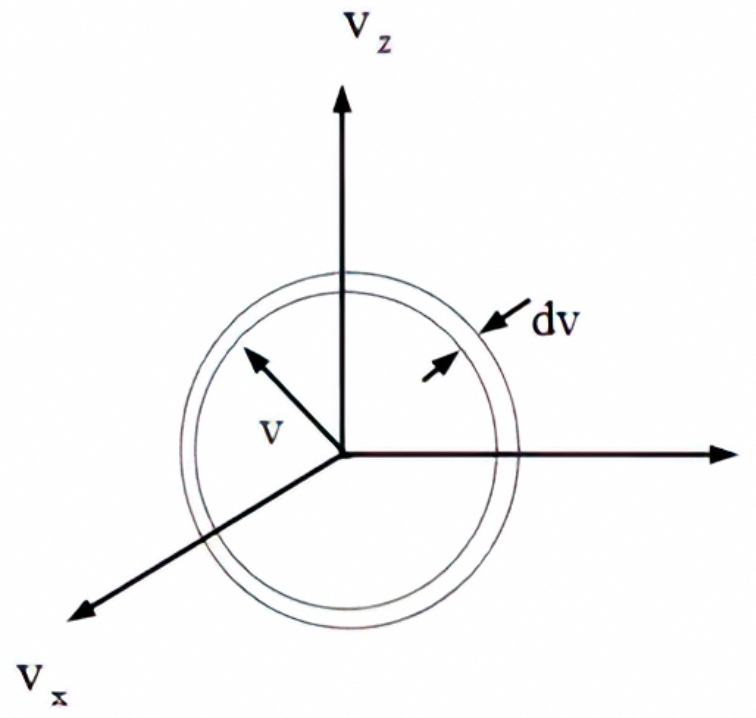
\includegraphics[scale=0.33]{1}
	\end{center}
	\caption{Пространство скоростей}
\end{figure}	

И таким образом, мы имеем функцию распределения $F(v)$:
\begin{equation}
F\left(v\right)=4\pi N{\left(\frac{m}{2\pi kT}\ \right) }^\frac{3}{2}e^{-\frac{mv^2}{kT}}v^2
\end{equation}

\begin{figure}[h!]
\begin{center}
	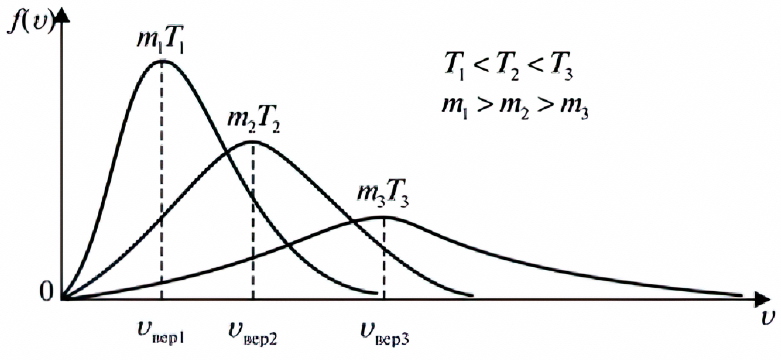
\includegraphics[scale=0.6]{2}
\end{center}
\caption{Распределение $f(v)$}
\end{figure}
Вид распределения Максвелла показан на рисунке. С увеличением температуры максимум распределения смещается в сторону больших скоростей, а высота кривой в максимуме несколько понижается.
Функция обращается в нуль при $v=0$ и при $v \rightarrow \infty$ так как неподвижных и движущихся бесконечно быстро молекул не бывает. Она имеет максимум при условии:
$$v= v_в=\sqrt{\frac{2kT}{m}}$$

\newpage
\subsection{Двумерное распределение}
\hspace{\parindent}Предположим, что молекулы могут двигаться только в координатах $x$ и $y$. Компонента скорости $v_z$ может быть любой. Мы ищем число молекул, компоненты $v_x$ и $v_y$ лежат в соответствующих для них интервалах. Проинтегрировав (18) по компоненте $v_z$ и обозначив $n= \sqrt{v_x^2+v_y^2}$, получаем:
\begin{equation}
dN^\prime=N\left(\frac{m}{2\pi kT}\right)e^{-\frac{mn^2}{kT}}dn_xdn_y,
\end{equation}
где $dn_x=dv_x$;$dn_y=dv_y$.

Молекулы будут находиться в бесконечно тонком кольце радиуса n и толщиной dn. Площадь данного кольца - $2\pi ndn$. Заменив $dn_xdn_y$ на данную площадь, получим:
\begin{equation}
dN^\prime=2\pi N\left(\frac{m}{2\pi kT}\right)e^{-\frac{mn^2}{kT}}ndn
\end{equation}

Для реального газа (22) представляет собой число молекул, у которых проекция на XY лежит в интервале от n до dn. Получаем функцию распределения:
\begin{equation}
F^\prime\left(n\right)=2\pi N\left(\frac{m}{2\pi kT}\right)e^{-\frac{mn^2}{kT}}n
\end{equation}

Возвращаемся к переменным v, дифференцируем (23) по v, приравнивая его к нулю. Получим наиболее вероятное значение вероятной скорости:
\begin{equation}
v_в=\sqrt{\frac{kT}{m}}
\end{equation}

Подставив (24) в (22), получим:
\begin{equation}
dN^\prime=\ Ne^{-\frac{mv^2}{kTv_в^2}}\frac{v}{v_в^2}dv 
\end{equation}

Проинтегрировав (25), получим:
\begin{equation}
\Delta N=N\bigg\{e^{-\frac{v_1^2}{2v_в^2}}- e^{-\frac{v_2^2}{2v_в^2}} \bigg\}     
\end{equation}
Это наша рабочая формула.

Т.к. мы не имеем возможности измерить скорость каждого зерна отдельно, приведем рабочую формулу к виду:
\begin{equation}
\Delta m_i=m\bigg[e^{-\frac{(i-1)^2}{2i_в^2}}- e^{-\frac{-i^2}{2iв2}}\bigg]
\end{equation}







\end{document}
